\documentclass[11pt,a4paper]{article}

\usepackage[T1]{fontenc}
\usepackage{lmodern}
\usepackage{microtype}
\usepackage[margin=2.4cm]{geometry}
\usepackage{amsmath,amssymb}
\usepackage{booktabs,tabularx}
\usepackage{enumitem}
\usepackage{tocloft}
\setlength{\cftbeforesecskip}{1pt}
\setlength{\cftbeforetoctitleskip}{0.6em}
\setlength{\cftaftertoctitleskip}{0.4em}
\usepackage{xcolor}
\usepackage{tikz}
\usetikzlibrary{arrows.meta,positioning,calc,fit}
\usepackage[skins,breakable]{tcolorbox}
\usepackage[colorlinks=true,linkcolor=blue!50!black,urlcolor=blue!50!black,citecolor=blue!50!black]{hyperref}

\setlength{\parskip}{0.55em}
\setlength{\parindent}{0pt}
\setlist{itemsep=0.2em,topsep=0.3em}
\renewcommand{\arraystretch}{1.25}

% ---------- boxes ----------
\definecolor{keyc}{HTML}{1F5FA8}
\definecolor{plainc}{HTML}{2E7D32}
\definecolor{warnc}{HTML}{B26A00}
\newtcolorbox{keyidea}[1][Key idea]{enhanced,colback=keyc!5,colframe=keyc,
  fonttitle=\bfseries,title=#1,boxrule=0.6pt,arc=2pt,left=6pt,right=6pt,top=4pt,bottom=4pt}
\newtcolorbox{plain}[1][In plain words]{enhanced,colback=plainc!5,colframe=plainc,
  fonttitle=\bfseries,title=#1,boxrule=0.6pt,arc=2pt,left=6pt,right=6pt,top=4pt,bottom=4pt}
\newtcolorbox{careful}[1][Be careful]{enhanced,breakable,colback=warnc!6,colframe=warnc,
  fonttitle=\bfseries,title=#1,boxrule=0.6pt,arc=2pt,left=6pt,right=6pt,top=4pt,bottom=4pt}

% ---------- notation ----------
\newcommand{\M}{\mathcal{M}}
\newcommand{\Lt}{\tilde{\mathcal{L}}}
\newcommand{\Lc}{\mathcal{L}}
\newcommand{\bk}{\mathbf{k}}
\newcommand{\bv}{\mathbf{v}}
\newcommand{\bq}{\mathbf{q}}
\newcommand{\bx}{\mathbf{x}}
\newcommand{\by}{\mathbf{y}}
\newcommand{\bm}{\mathbf{m}}
\newcommand{\inner}[2]{\langle #1, #2\rangle}

\title{\textbf{Nested Learning, Explained Simply}\\[0.3em]
\large A study guide to \emph{Nested Learning: The Illusion of Deep Learning Architectures}\\
(Behrouz, Razaviyayn, Zhong, Mirrokni; NeurIPS 2025, arXiv:2512.24695)}
\author{Prepared for Harsh Chattar}
\date{27 October 2026}

\begin{document}
\maketitle

\begin{keyidea}[The whole paper in five sentences]
\begin{enumerate}[leftmargin=1.4em]
  \item A neural network \emph{and} its optimizer can be described as a set of small optimization problems stacked inside each other. Each one has its own data (its \emph{context flow}) and its own update speed (its \emph{frequency}).
  \item Every one of these small problems is an \textbf{associative memory}: something that learns to map keys to values by gradient descent. Attention, linear attention, MLP layers, momentum and Adam all fit this mould.
  \item So the ``architecture'' we draw on paper is only the flattened picture. The real structure is a ladder of \textbf{levels} ordered by update frequency. Seeing only the flat picture is the ``illusion'' in the title.
  \item This view suggests a new design axis: add \emph{more levels}, i.e.\ more parts that learn at different speeds. That should help continual learning, because knowledge lives at several time scales.
  \item The paper builds three things on this idea: more expressive optimizers (Delta GD, M3), the \textbf{Continuum Memory System (CMS)} of MLPs at many speeds, and \textbf{Hope}, a self-modifying sequence model with CMS.
\end{enumerate}
\end{keyidea}

\setcounter{tocdepth}{1}
\tableofcontents
\newpage

% =====================================================================
\section{The problem NL wants to fix}

\paragraph{Today's models stop learning after training.}
A large language model (LLM) learns during pre-training. After that its weights are frozen. The only thing that still adapts is \emph{in-context learning}: the model can use what is in its current prompt. Once the prompt is gone, so is that knowledge.

The authors compare this to \textbf{anterograde amnesia}. A patient with this condition keeps their old memories but cannot form new long-term ones. They live in a short window of ``now'' plus the distant past. An LLM is similar:
\begin{itemize}
  \item the \emph{distant past} is what was stored in its MLP weights before ``the end of pre-training'';
  \item the \emph{now} is its context window (attention);
  \item nothing moves from ``now'' into long-term storage.
\end{itemize}

\paragraph{What the brain does differently.}
The paper borrows two ideas from neuroscience.
\begin{enumerate}
  \item \textbf{Many time scales.} Brain activity runs at several frequencies at once (fast gamma waves, slower beta, very slow delta/theta). Fast ones handle sensory input; slow ones are linked to memory consolidation. In a standard network, in contrast, every layer is updated at the same rate during training and at rate zero afterwards.
  \item \textbf{Uniform, reusable structure.} Brain tissue is not rigidly split into ``short-term memory here, long-term memory there''. Memory is distributed and the same kind of tissue is reused for different jobs.
\end{enumerate}

\begin{plain}
NL asks: what if parts of a model learned at different speeds, all the time, the way the brain consolidates memories? To even talk about this, we need a language in which ``update speed'' is a first-class property of every component. That language is Nested Learning.
\end{plain}

% =====================================================================
\section{The building block: associative memory}

\subsection{Definition}
\textbf{Definition (associative memory).} Given keys $K$ and values $V$, an associative memory is an operator $\M(\cdot)$ that maps keys to values. It is found by minimising some objective $\Lt$ that measures how good the mapping is:
\begin{equation}
  \M^{*} = \arg\min_{\M}\ \Lt\big(\M(K);\,V\big).
\end{equation}
Keys and values do not have to be tokens. They can be gradients, data points, error signals, anything.

The paper also fixes two words, taken from neuropsychology:
\begin{itemize}
  \item \textbf{Memory} is a neural update caused by an input.
  \item \textbf{Learning} is the process of acquiring effective and useful memory.
\end{itemize}
So in NL, \emph{any} weight change caused by data is a memory.

\subsection{Familiar layers as associative memories}
Pick an objective $\Lt$ and an optimizer for it, and you get a known layer. Assume keys $\bk_t$, values $\bv_t$ and queries $\bq_t$ are given (they come from projections of the input).

\paragraph{Linear attention = gradient descent on a dot-product objective.}
Take a matrix memory $\M$ and $\Lt(\M;\bk,\bv) = -\inner{\M\bk}{\bv}$. Its gradient is $-\bv\bk^{\top}$. One gradient step with learning rate 1 gives
\begin{equation}
  \M_t = \M_{t-1} + \bv_t\bk_t^{\top},
\end{equation}
which is exactly the (unnormalised) linear attention / fast-weight update. Reading is $\by_t = \M_t\bq_t$.

\paragraph{Delta rule = gradient descent on a regression objective.}
Use $\Lt = \tfrac12\|\M\bk - \bv\|_2^2$ instead. The step becomes
\begin{equation}
  \M_t = \M_{t-1} - \eta_t(\M_{t-1}\bk_t - \bv_t)\bk_t^{\top}
       = \M_{t-1}\big(I - \eta_t\bk_t\bk_t^{\top}\big) + \eta_t\bv_t\bk_t^{\top}.
\end{equation}
The extra term $\M_{t-1}\bk_t\bk_t^{\top}$ \emph{erases} what the memory currently stores along $\bk_t$ before writing the new value. This is DeltaNet. It manages limited capacity better than the purely additive (Hebbian) rule.

\paragraph{Softmax attention = the exact, non-parametric solution.}
Weight each stored pair by a similarity $s(\bk_i,\bq)$ and solve a weighted regression:
\begin{equation}
  \M^{*}(\bq) = \arg\min_{\M}\sum_{i=1}^{L} s(\bk_i,\bq)\,\|\bv_i - \M\|_2^2
  = \sum_{i=1}^{L}\frac{s(\bk_i,\bq)}{\sum_{j} s(\bk_j,\bq)}\,\bv_i .
\end{equation}
With $s(\bk,\bq)=\exp(\bq^{\top}\bk)$ this is softmax attention. It is a \emph{non-parametric} memory: it does not compress the context into weights; it keeps all of it and solves the problem exactly for every query. Restricting the sum to the last $c$ tokens gives sliding-window attention.

\begin{plain}
Attention, linear attention and DeltaNet are not three unrelated inventions. They are the same thing, ``learn a key$\to$value map'', with a different objective and a different way of solving it.
\end{plain}

% =====================================================================
\section{Surprise: training itself is a memory}

The next step is the most surprising one in the paper: \emph{the training process} is also an associative memory.

\subsection{Backpropagation stores errors}
Take one linear layer $\by = W\bx$ trained with gradient descent. Let $\boldsymbol\delta_t = \nabla_{\by}\Lc$ be the gradient of the loss with respect to the layer's output. Then $\nabla_W\Lc = \boldsymbol\delta_t\bx_t^{\top}$ and
\begin{equation}
  W_{t+1} = W_t - \eta_{t+1}\,\boldsymbol\delta_{t+1}\bx_{t+1}^{\top}
  \;=\; \arg\min_{W}\ \inner{W\bx_{t+1}}{\boldsymbol\delta_{t+1}} + \frac{1}{2\eta_{t+1}}\|W - W_t\|_2^2 .
\end{equation}
Read the right-hand side as a memory problem. The layer is learning a map from each input $\bx$ to its error signal $\boldsymbol\delta$, while staying close to its previous state. The paper calls $\boldsymbol\delta$ the \textbf{Local Surprise Signal (LSS)}: how surprising the layer's output was for this input. It is zero when the loss is minimised.

\begin{keyidea}[Backprop as a surprise-based memory]
A network trained by backpropagation learns by memorising how surprising its predictions were. Each layer stores a mapping from its inputs to its local error signals.
\end{keyidea}

One subtlety: the values $\boldsymbol\delta$ depend on the current weights, so the memory \emph{generates its own values}. The paper calls this a \textbf{self-referential} process. It is why gradient descent is richer than ``linear attention on gradients''.

\subsection{Momentum is a second, faster memory}
Gradient descent with momentum is
\begin{equation}
  W_{t+1} = W_t + \bm_{t+1},\qquad \bm_{t+1} = \alpha_{t+1}\bm_t - \eta_{t+1}\nabla\Lc(W_t;\bx_{t+1}).
\end{equation}
The momentum update is one gradient step on the objective $\min_{\bm}\inner{\bm}{\nabla\Lc}$ (with $\alpha$ acting as a retention or weight-decay term). So:
\begin{itemize}
  \item the \textbf{inner} problem: the momentum $\bm$ learns to compress past gradients;
  \item the \textbf{outer} problem: the weights $W$ are updated using what the momentum stored.
\end{itemize}
Plain SGD is a one-level memory. SGD with momentum is a \emph{two-level} nested system.

\subsection{Other optimizers}
The same reading works for the rest of the optimizer zoo.
\begin{itemize}
  \item \textbf{Adam} (with RMSProp, AdaGrad, Lion, \dots) are associative memories over gradients. The paper argues Adam is the \emph{optimal} memory for an element-wise $\ell_2$ regression objective over gradient statistics.
  \item \textbf{Preconditioning} (Shampoo, Soap) learns a map from gradients into a better coordinate system. That map is itself a memory.
  \item \textbf{Muon} applies Newton--Schulz iterations to the momentum. Each iteration is a gradient step on an objective that pushes the output towards an orthogonal matrix. So Muon hides one more inner optimization problem.
\end{itemize}

\subsection{Why plain momentum is a short memory}
With momentum decay $\beta=0.9$, a gradient $j$ steps old has weight proportional to $\beta^{j}$. The share of the last $n$ gradients is $1-\beta^{n}$:
\[
 1-0.9^{7}\approx 0.52,\qquad 1-0.9^{44}\approx 0.99 .
\]
So about the last 7 gradients carry half the weight and about the last 44 carry 99\%. Momentum is a low-pass filter with a very short memory. In continual learning this matters: after a long stretch on task $B$, the optimizer has no memory of which directions were important for task $A$, so it happily moves weights in directions that damage $A$. This motivates optimizers with a longer, multi-scale memory (Section~\ref{sec:m3}).

% =====================================================================
\section{Levels and update frequency}

\subsection{Frequency}
\textbf{Definition (update frequency).} Let one update step on one data point be one unit of time. The frequency $f_A$ of a component $A$ is its number of updates per unit of time.

Components are then ordered:
\begin{itemize}
  \item $A$ is \emph{faster} than $B$ if $f_A > f_B$;
  \item or if $f_A = f_B$ but computing $B$'s state at time $t$ needs $A$'s state at time $t$ (e.g.\ the weight update needs the momentum first, so momentum is the faster one).
\end{itemize}
Components with the same frequency share a \textbf{level}. Higher levels are slower.

\subsection{Nested system}
\textbf{Definition (nested system).} A system with $K$ ordered levels. Each level holds one or more optimization problems, each described by three things:
\begin{center}
\begin{tabular}{ll}
  $\Lc$ & its objective,\\
  $C$ & its context (the data it is optimized on),\\
  $\Theta$ & its parameters,
\end{tabular}
\end{center}
and each is solved by (some form of) gradient descent. \textbf{Each problem has its own gradient flow}: a separate ``box'' of optimization. If every context is a set of key--value pairs, the system is a \emph{Nested System of Associative Memories (NSAM)}. The paper's examples are all NSAMs.

\subsection{A Transformer through NL glasses}
\begin{center}
\begin{tabularx}{\textwidth}{lXl}
\toprule
\textbf{Component} & \textbf{What it compresses (its context)} & \textbf{Frequency}\\
\midrule
Attention & the tokens of the current sequence; solved exactly for every token & $\infty$ (every token)\\
Optimizer state (momentum, Adam) & the gradients produced by the network & every training step\\
Projections $W_Q,W_K,W_V$, MLPs & the whole pre-training dataset & every step in training, \textbf{0} after\\
\bottomrule
\end{tabularx}
\end{center}
So a deployed Transformer has only two extreme frequencies: $\infty$ for attention and $0$ for everything else. Nothing lives in between. That gap is exactly the ``amnesia'' of Section~1.

\begin{figure}[h]
\centering
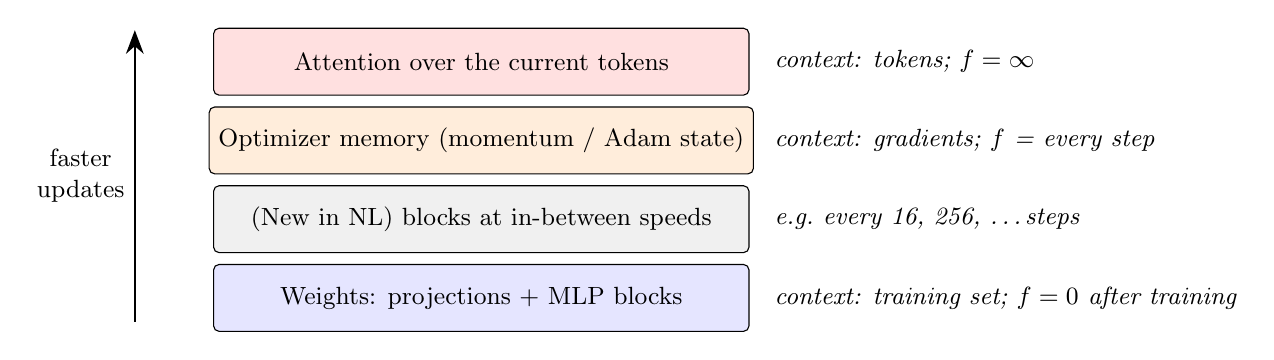
\begin{tikzpicture}[
  lvl/.style={draw,rounded corners=2pt,minimum width=6.8cm,minimum height=0.85cm,align=center,font=\small},
  lab/.style={font=\small\itshape,align=left,anchor=west}]
  \node[lvl,fill=red!12]   (a) at (0,3.0) {Attention over the current tokens};
  \node[lvl,fill=orange!14](b) at (0,2.0) {Optimizer memory (momentum / Adam state)};
  \node[lvl,fill=blue!10]  (c) at (0,0.0) {Weights: projections + MLP blocks};
  \node[lvl,fill=gray!12]  (d) at (0,1.0) {(New in NL) blocks at in-between speeds};
  \draw[-{Stealth[length=3mm]},thick] (-4.4,-0.3) -- (-4.4,3.4) node[midway,left,align=center,font=\small]{faster\\updates};
  \node[lab] at (3.6,3.0) {context: tokens; $f=\infty$};
  \node[lab] at (3.6,2.0) {context: gradients; $f$ = every step};
  \node[lab] at (3.6,0.0) {context: training set; $f=0$ after training};
  \node[lab] at (3.6,1.0) {e.g.\ every 16, 256, \dots steps};
\end{tikzpicture}
\caption{Levels of a Transformer + optimizer. Standard models only use the extremes. NL proposes filling the gap with components that update at intermediate frequencies (grey row).}
\end{figure}

\begin{keyidea}[Why ``the illusion of deep learning architectures'']
If you open every box, every component is just a linear layer or MLP solving its own regression problem at its own speed. Attention looks different from an MLP only because we see the \emph{solution} of its inner problem, not the problem. The visible heterogeneity of architectures is an artefact of looking at a flattened picture. NL claims that the real extra dimension is the number of \emph{levels}, not the number of layers.
\end{keyidea}

% =====================================================================
\section{How levels pass knowledge to each other}

Having levels is not enough; they must talk. The paper lists the main channels between a faster block and a slower one:

\begin{center}
\begin{tabularx}{\textwidth}{@{}>{\raggedright}p{2.9cm}X>{\raggedright\arraybackslash}p{4.2cm}@{}}
\toprule
\textbf{Channel} & \textbf{How it works} & \textbf{Known example}\\
\midrule
Direct, parametric & The slow block's output is conditioned on the fast block's parameters or output. No gradient flows between them. & Linear attention / fast weights\\
Direct, non-parametric & The slow block's output is conditioned on the fast block's raw context. & Softmax attention\\
Via backpropagation & Both blocks sit in one gradient flow but are updated at different rates. & CMS (Section~\ref{sec:cms})\\
Via initialization & The slow level learns the \emph{starting point} of the fast level. & MAML, meta-learned memory $\M_0$\\
Via generation & One block generates the weights or the input of another. & Hypernetworks; the network generating gradients for the optimizer\\
\bottomrule
\end{tabularx}
\end{center}

\begin{keyidea}[NL's design recipe]
To design a model in NL you make two choices:
\begin{enumerate}[leftmargin=1.4em]
  \item which optimization problems exist and at what frequency each one runs;
  \item how knowledge transfers between the levels.
\end{enumerate}
Meta-learning, MAML, hypernetworks, learned optimizers and fast-weight RNNs are all particular answers to these two questions.
\end{keyidea}

A neat example from the paper: replace an MLP in a Transformer by linear attention whose \emph{initial} memory state $\M_0$ is meta-learned (they call it ``AdaTransformer''). The two blocks look almost the same. The only difference is that the linear-attention block has a second, faster level that adapts to the current sequence, starting from a learned $\M_0$. In other words, \emph{a recurrent memory is an MLP with one extra level added}.

% =====================================================================
\section{Familiar terms, re-read through NL}

This is the ``philosophy'' part of the paper. These points come up often in discussions, so they are worth knowing.

\begin{description}[style=nextline,leftmargin=0pt]
  \item[In-context learning (ICL) is a consequence of having levels.]
  NL defines ICL broadly: any adaptation of a component to its own context. Every level does ICL on its own context flow. So ICL is not a mysterious emergent property; it follows from the multi-level structure. It still needs a strong slow level, or the fast level has too little to work with.

  \item[Pre-training is ICL with a huge context.]
  The slowest level's context is the entire pre-training set. Pre-training is that level compressing its context into its weights.

  \item[Test-time training is parametric ICL.]
  Methods like TTT and Titans compress the current context into memory weights. When the context goes, that knowledge goes too, unless it is transferred to a slower level.

  \item[There is no real train/test boundary.]
  A model is always either receiving input or isolated. ``End of pre-training'' just means we cut the knowledge transfer from fast levels to slow ones.

  \item[Models have more parameters than we think.]
  Optimizer states and RNN hidden states also store knowledge (about the loss landscape, about the context). When training ends, the optimizer state is thrown away, and with it what it knew.

  \item[Architecture and optimizer are one system.]
  The architecture generates the optimizer's data (its gradients). So the best optimizer depends on the architecture. NL argues for \emph{architecture-specific optimizers}.

  \item[Hybrid models are Transformers with extra levels.]
  Adding a recurrent memory to a Transformer is adding a level to some MLP blocks, not mixing two different species.
\end{description}

% =====================================================================
\section{What NL builds: more expressive optimizers}

Once momentum and gradient descent are seen as memories, one can upgrade them the same way sequence models were upgraded from linear attention to DeltaNet and to deep memories.

\begin{itemize}
  \item \textbf{More expressive association.} Let momentum map keys to values instead of just accumulating gradients. This gives a preconditioned momentum.
  \item \textbf{Delta Momentum.} Replace the dot-product inner objective by $\ell_2$ regression. The momentum update then depends on its own state and can \emph{forget} stale gradients. In a toy problem with a fast-changing landscape, it converges faster than standard momentum.
  \item \textbf{Deep Momentum GD (DMGD).} Replace the momentum matrix by a small MLP, for more capacity.
  \item \textbf{Nonlinear outputs.} Apply a nonlinearity to the momentum's output. Choosing Newton--Schulz here recovers Muon.
\end{itemize}

\subsection{Delta Gradient Descent (DGD)}\label{sec:dgd}
Plain gradient descent treats each sample independently of the current weights. That is fine for i.i.d.\ data but not for correlated streams such as tokens. Replacing the inner dot-product objective by $\ell_2$ regression, with normalised inputs ($\|\bx_t\|=1$), gives
\begin{equation}
  W_{t+1} = W_t\big(I - \eta'_t\,\bx_t\bx_t^{\top}\big) - \eta'_t\,\nabla_{\by}\Lc(W_t;\bx_t)\,\bx_t^{\top}.
\end{equation}
The first term is an \emph{input-dependent decay}: the step first erases what $W$ currently does along $\bx_t$, then writes. It is the delta rule applied to the weights themselves. Hope uses DGD inside its memories.

\paragraph{Generalized Gradient Descent (GGD).} More generally, NL defines gradient descent as any self-referential memory that maps inputs to \emph{values it generates itself}, plus a retention term that keeps the new state close to the old one. Plain GD and DGD are two instances.

% =====================================================================
\section{The Continuum Memory System (CMS)}\label{sec:cms}

CMS is the part of NL that is easiest to implement and the main tool for continual learning.

\subsection{From two memories to a spectrum}
Usual designs have a short-term memory (attention) and a long-term one (MLPs). CMS replaces this pair with a \emph{spectrum}: a chain of MLP blocks, each updated at its own frequency.

\begin{equation}
  \by_t = \mathrm{MLP}^{(f_k)}\Big(\mathrm{MLP}^{(f_{k-1})}\big(\cdots\mathrm{MLP}^{(f_1)}(\bx_t)\big)\Big).
\end{equation}
Block $\ell$ has a chunk size $C^{(\ell)}$ (smaller for faster blocks). Its parameters change only once every $C^{(\ell)}$ steps, using the error terms accumulated over that chunk:
\begin{equation}
  \theta^{(f_\ell)}_{i+1} =
  \begin{cases}
    \theta^{(f_\ell)}_{i} - \displaystyle\sum_{t=i-C^{(\ell)}}^{i}\eta_t^{(\ell)}\, f\big(\theta_t^{(f_\ell)};\bx_t\big) & \text{if } i \equiv 0 \pmod{C^{(\ell)}},\\[1.2em]
    \theta^{(f_\ell)}_{i} & \text{otherwise.}
  \end{cases}
\end{equation}
Here $f(\cdot)$ is the error term of whatever optimizer is used (for SGD, the gradient of the \emph{task} loss). In practice this is \textbf{gradient accumulation with a different period per block}.

A standard Transformer MLP is the special case with one block ($k=1$) and frequency 0 after training.

\begin{figure}[h]
\centering
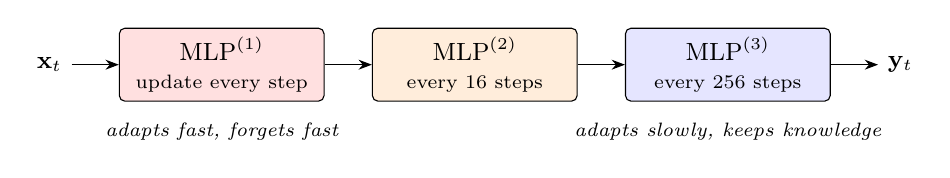
\begin{tikzpicture}[
  blk/.style={draw,rounded corners=2pt,minimum width=2.6cm,minimum height=0.9cm,font=\small,align=center},
  >=Stealth]
  \node[font=\small] (in) at (0,0) {$\bx_t$};
  \node[blk,fill=red!12,right=0.6cm of in]   (m1) {MLP$^{(1)}$\\[-1pt]\scriptsize update every step};
  \node[blk,fill=orange!14,right=0.6cm of m1](m2) {MLP$^{(2)}$\\[-1pt]\scriptsize every 16 steps};
  \node[blk,fill=blue!10,right=0.6cm of m2]  (m3) {MLP$^{(3)}$\\[-1pt]\scriptsize every 256 steps};
  \node[font=\small,right=0.6cm of m3] (out) {$\by_t$};
  \draw[->] (in) -- (m1); \draw[->] (m1) -- (m2); \draw[->] (m2) -- (m3); \draw[->] (m3) -- (out);
  \node[font=\scriptsize\itshape,below=0.15cm of m1] {adapts fast, forgets fast};
  \node[font=\scriptsize\itshape,below=0.15cm of m3] {adapts slowly, keeps knowledge};
\end{tikzpicture}
\caption{A sequential CMS with three blocks. The frequencies are only an illustration.}
\end{figure}

\subsection{Three ways to wire the blocks}
\begin{itemize}
  \item \textbf{Nested CMS.} Level $\ell$ meta-learns the \emph{initial state} of level $\ell+1$. Level $\ell+1$ is reset to that start after each of its contexts. This gives ``higher-order'' in-context learning.
  \item \textbf{Sequential CMS.} The blocks run in series (as in the figure). All initial states are learned by backprop at the slowest level.
  \item \textbf{Independent (head-wise) CMS.} The blocks run in parallel on the same input and their outputs are combined: $\by_t = \mathrm{Agg}\big(\mathrm{MLP}^{(f_k)}(\bx_t),\dots,\mathrm{MLP}^{(f_1)}(\bx_t)\big)$, for example a learnable weighted sum.
\end{itemize}

\subsection{Why CMS should reduce forgetting}
Forgetting happens when updating a block overwrites what it stored. In CMS, when a fast block overwrites something, the slower blocks still hold it. Because all blocks share one gradient flow, backprop can carry that knowledge back into the fast block later. Knowledge can thus \emph{loop} through time instead of being lost.

\subsection{Is it expensive?}
Not much. At any step only the blocks whose period has come up are updated. Inside a chunk there is no sequential dependency, so the work can be parallelised.

\subsection{Starting from a pretrained model}
NL suggests \textbf{initialising every CMS block from a pretrained model's MLP}: $\mathrm{MLP}^{(\ell)}_0 = \mathrm{MLP}_{\text{pre-trained}}$. The learning rate of each level controls how far it may drift. As $\eta^{(\ell)}\to 0$ the block stays at the pretrained weights. This ``ad-hoc level stacking'' turns an existing model (the paper uses Llama-3) into a multi-level one without training from scratch.

% =====================================================================
\section{M3: CMS inside the optimizer}\label{sec:m3}

\textbf{Multi-scale Momentum Muon (M3)} applies the CMS idea to the optimizer's memory. It is a proof of concept that CMS works for a different context flow (gradients instead of tokens). In short, M3 = Adam + Muon + a two-level CMS on the momentum.

\begin{tcolorbox}[colback=gray!4,colframe=gray!60,title=\textbf{M3, one step for a weight matrix $W$} (paper's Algorithm~1),fonttitle=\small,boxrule=0.5pt,arc=2pt]
\small
\begin{tabular}{@{}ll@{}}
Gradient & $g_t = \nabla_W \Lc(W_t)$\\
Fast momentum (every step) & $M^{(1)}_t = \beta_1 M^{(1)}_{t-1} + g_t$\\
Second moment (every step, as in Adam) & $V_t = \beta_2 V_{t-1} + (1-\beta_2)\,g_t^{2}$\\
Slow momentum (every $\hat f$ steps only) & $M^{(2)} \leftarrow \beta_3 M^{(2)} + \sum_{\text{last }\hat f\text{ steps}} g$\\
Orthogonalise both (as in Muon) & $O^{(1)} = \mathrm{NS}(M^{(1)}_t),\quad O^{(2)} = \mathrm{NS}(M^{(2)})$\\
Update & $W_{t+1} = W_t - \eta\,\dfrac{O^{(1)} + \alpha\,O^{(2)}}{\sqrt{V_t}+\epsilon}$
\end{tabular}

\smallskip
NS = Newton--Schulz orthogonalisation. $\alpha$ weights the slow memory; $\alpha=0$ removes the NL part.
\end{tcolorbox}

The slow momentum $M^{(2)}$ sees a summary of many more past gradients than ordinary momentum, so it should give the optimizer a longer view of the loss landscape. The paper notes that M3 adds overhead and may be harder to scale. The algorithm in the paper writes the $\beta$'s as plain additions; the decaying form above is the usual reading. No hyperparameter values are given.

% =====================================================================
\section{Titans, self-modifying Titans and Hope}

\subsection{Titans in brief}
Titans (Behrouz et al., 2025) is the precursor of Hope. It is a sequence model with a \textbf{neural long-term memory} $\M$ (a small MLP) that is trained \emph{while reading the sequence}:
\begin{align}
  \bk_t &= \bx_tW_K,\quad \bv_t = \bx_tW_V, & \ell(\M_{t-1};\bx_t) &= \|\M_{t-1}(\bk_t)-\bv_t\|_2^2,\\
  S_t &= \eta_t S_{t-1} - \theta_t\nabla\ell(\M_{t-1};\bx_t), & \M_t &= (1-\alpha_t)\M_{t-1} + S_t .
\end{align}
\begin{itemize}
  \item $\nabla\ell$ is the \textbf{surprise}: how badly the memory predicted this input. Big surprise means a big write.
  \item $S_t$ is a \textbf{momentum of surprise}, so an event stays ``surprising'' for a while.
  \item $\alpha_t$ is a \textbf{forget gate} (weight decay).
  \item $\eta_t,\theta_t,\alpha_t$ depend on the input. They, $W_K$, $W_V$ and the starting memory $\M_0$ are learned in the outer loop.
\end{itemize}
Reading is a plain forward pass: $\by_t = \M_t(\bq_t)$. In NL terms Titans has two levels: the memory (fast, per token) and everything else (slow, pre-training).

\subsection{Self-modifying (self-referential) Titans}
In Titans the projections that produce $\bk,\bv$ and the rates $\eta,\alpha$ are frozen after training. So the model's way of \emph{reading} its input cannot adapt to the context. NL's fix is to make each of them a memory too:
\begin{align}
  \bk_t &= \M_{k,t-1}(\bx_t),\ \ \bv_t = \M_{v,t-1}(\bx_t),\ \ \eta_t = \M_{\eta,t-1}(\bx_t),\ \ \alpha_t = \M_{\alpha,t-1}(\bx_t),\ \ \bq_t = \bx_tW_q,\\
  \hat\bv_{\square,t} &= \M_{\square,t-1}(\bv_t) \qquad\text{(each memory generates its own target value)},\\
  \M_{\square,t} &= \M_{\square,t-1}\big(\alpha_t I - \eta_t\bk_t\bk_t^{\top}\big) - \eta_t\nabla\Lc\big(\M_{\square,t-1};\bk_t,\hat\bv_{\square,t}\big),
\end{align}
for $\square\in\{k,v,\eta,\alpha,\text{memory}\}$, and the output is $\by_t = \M_{\text{memory},t-1}(\bq_t)$.
\begin{itemize}
  \item Only the query projection $W_q$ stays fixed.
  \item Each memory is a residual 2-layer MLP: $\M(\bx) = \bx + W_1\sigma(W_2\bx)$.
  \item Updates use DGD with weight decay (Section~\ref{sec:dgd}).
  \item All initial states $\M_{\square,0}$ are meta-learned in the outer loop.
  \item \textbf{Chunked training}: inside a chunk, all gradients are taken with respect to the state at the end of the previous chunk. So a chunk is processed in parallel.
\end{itemize}
``Self-modifying'' means the model learns how to change its own projections and learning rates, not just its memory contents.

\subsection{Hope}
\begin{keyidea}[Hope = self-modifying Titans $\rightarrow$ CMS]
Each Hope block is a self-modifying Titans layer followed by a Continuum Memory System. The two are complementary:
\begin{itemize}[leftmargin=1.2em]
  \item self-modifying Titans: \emph{small capacity, expressive learning rule}, fast adaptation to the context;
  \item CMS: \emph{large capacity, simple learning rule}, persistent knowledge at many time scales.
\end{itemize}
\textbf{Hope-Attention} is the variant that uses ordinary softmax attention in place of the self-modifying Titans, followed by CMS.
\end{keyidea}

% =====================================================================
\section{What the paper shows experimentally}

All main experiments are on language. The headline claims:
\begin{itemize}
  \item \textbf{Class-incremental learning} (text intent / topic classification: CLINC, Banking, DBpedia). Llama-3 (3B and 8B) MLPs were turned into CMS blocks with pretrained initialisation, then continually pre-trained on 15B tokens. This beat plain ICL, EWC and InCA (a continual learner with an external module).
  \item \textbf{More levels help continual learning}. More levels and a well-chosen lowest frequency improve continual and in-context learning. A very fast lowest frequency adapts well but keeps less long-term knowledge.
  \item \textbf{Long context} (needle-in-a-haystack, BABILong): Hope trained from scratch on about 50B tokens, compared with recurrent and deep-memory models (RetNet, DeltaNet, RWKV-7, Comba, Titans, \dots).
  \item \textbf{Language modelling and common-sense reasoning} at 760M parameters / 30B tokens and 1.3B / 100B tokens: Hope is competitive as a general backbone.
  \item \textbf{In-context recall}: Transformers remain best; Hope beats the attention-free models and narrows the gap.
  \item \textbf{Ablations}: replacing DGD by plain GD, removing momentum, removing weight decay, removing CMS, or freezing the $k,v,q$ projections all hurt.
  \item \textbf{M3 optimizer}: the \emph{only vision result}. A ViT (24M and 86M parameters) trained on ImageNet-21K reaches lower train and test loss with M3 than with AdamW or Muon. M3 is slower than Muon and on par with AdaMuon in speed.
\end{itemize}

\begin{careful}[What the authors themselves say]
They do not claim catastrophic forgetting is solved. In NL's view forgetting is a natural consequence of compression: a network of limited capacity must forget to make room. They present NL as ``a roadmap rather than a destination'': progress should come from exploiting the new axis of \emph{levels} rather than ever-deeper static networks.
\end{careful}

% =====================================================================
\section{A critical reading (useful for discussion)}

\begin{itemize}
  \item \textbf{Mostly a viewpoint.} Much of the paper re-describes known things (attention, momentum, Adam, MAML) in one language. That is valuable for intuition, but the reinterpretation alone does not improve any model. The new, testable pieces are DGD, CMS, M3, self-modifying Titans and Hope.
  \item \textbf{Mostly language.} Continual-learning evidence is on text classification with LLMs. The only vision evidence is the M3 loss curves on ImageNet-21K; it reports loss, not downstream accuracy.
  \item \textbf{Many design choices left open.} Frequencies, chunk sizes, how to aggregate CMS blocks, and M3's hyperparameters are not prescribed. A practitioner must choose them.
  \item \textbf{No official code} was available when we checked (October 2026), so implementations follow the equations in the paper.
\end{itemize}

% =====================================================================
\section{Cheat sheet}

\begin{center}
\begin{tabularx}{\textwidth}{@{}lX@{}}
\toprule
\textbf{Term} & \textbf{One-line meaning}\\
\midrule
Associative memory & Anything that learns a key$\to$value map by minimising an objective.\\
Context flow & The data a given component is optimized on (tokens, gradients, the training set, \dots).\\
Update frequency & How many times a component updates per data point.\\
Level & A group of components with the same update frequency; higher level = slower.\\
Nested system / NSAM & A model described as levels of optimization problems, each with its own gradient flow.\\
Local Surprise Signal & $\nabla_{\by}\Lc$: the error at a layer's output; what backprop ``stores''.\\
Surprise (Titans) & Gradient of the memory's loss on a new input; big when the input is unexpected.\\
Knowledge transfer & How levels influence each other: direct, backprop, initialization, generation.\\
Delta rule & Regression-based memory update that erases along the key before writing.\\
DGD & Delta rule applied to the network's own weights.\\
CMS & A chain (or set) of MLPs, each updated at its own frequency.\\
M3 & Adam + Muon + a fast and a slow momentum (CMS in the optimizer).\\
Self-modifying Titans & Titans where projections and learning rates are themselves memories that adapt in context.\\
Hope & Self-modifying Titans followed by CMS. Hope-Attention: softmax attention followed by CMS.\\
\bottomrule
\end{tabularx}
\end{center}

% =====================================================================
\section{Questions you may be asked, with short answers}

\begin{description}[style=nextline,leftmargin=0pt]
  \item[Is Nested Learning an architecture or a way of looking at models?]
  Mainly a way of looking at models (a paradigm). It also produces concrete designs: DGD, CMS, M3, self-modifying Titans and Hope.

  \item[What exactly is ``nested''?]
  Optimization problems. Inside the training loop there are other, faster optimization problems: the momentum learning gradients, attention solving a regression per token, a memory learning per sequence. Each has its own data and its own speed.

  \item[Why is the paper called ``the illusion of deep learning architectures''?]
  Because when you open the boxes, every component is a feedforward layer optimizing its own objective at its own speed. Architectures only look different because we see the solutions of these inner problems, not the problems themselves.

  \item[How is CMS different from just using different learning rates per layer?]
  A learning rate changes the \emph{size} of each step. CMS changes \emph{how often} a block steps, and accumulates the error over the whole period. A slow block therefore sees a summary of a long stretch of data, which is what lets it keep longer-term knowledge.

  \item[How does NL relate to meta-learning and MAML?]
  MAML is one special case: two levels where the slow level learns the initialization of the fast level (``knowledge transfer via initialization'').

  \item[How does NL relate to Titans?]
  Same first author. Titans is a two-level memory model; NL generalises it, explains it as an associative memory, and extends it to self-modifying Titans and Hope.

  \item[Why should multiple speeds help continual learning?]
  Fast parts adapt to new data; slow parts keep old knowledge because they change rarely and only in an averaged way. Knowledge lost in a fast part can be recovered from the slow parts through backprop.

  \item[What evidence is there outside language?]
  Only the M3 optimizer on ImageNet-21K (training and test loss for a ViT). The continual-learning and Hope results are all on text.
\end{description}

\end{document}
